\chapter{Patterns}
\input{Patterns/Prefix-Sum Pattern}
303, 525, 560

\chapter{Prefix - Suffix Product}
\section{Questions}\\


\href{https://leetcode.com/problems/product-of-array-except-self/description/}{238. Product of Array Except Self}


\section{Example Usage}\\



\begin{lstlisting}
 public int[] ProductExceptSelf(int[] nums) {
        var prefix = new int[nums.Length];
        var suffix = new int[nums.Length];
        var result = new int[nums.Length];

				prefix[0]=1;
        for(int i = 1; i<nums.Length; i++){
					prefix[i]=prefix[i-1]*nums[i-1];
        }


        suffix[nums.Length-1]=1;

        for(int j=nums.Length-2; j>= 0; j--){
            suffix[j]=suffix[j+1] * nums[j+1];
        }


        for(int i = 0; i<nums.Length; i++){
            result[i] = prefix[i]*suffix[i];
        }
        return result;
    }
		
\begin{figure}
		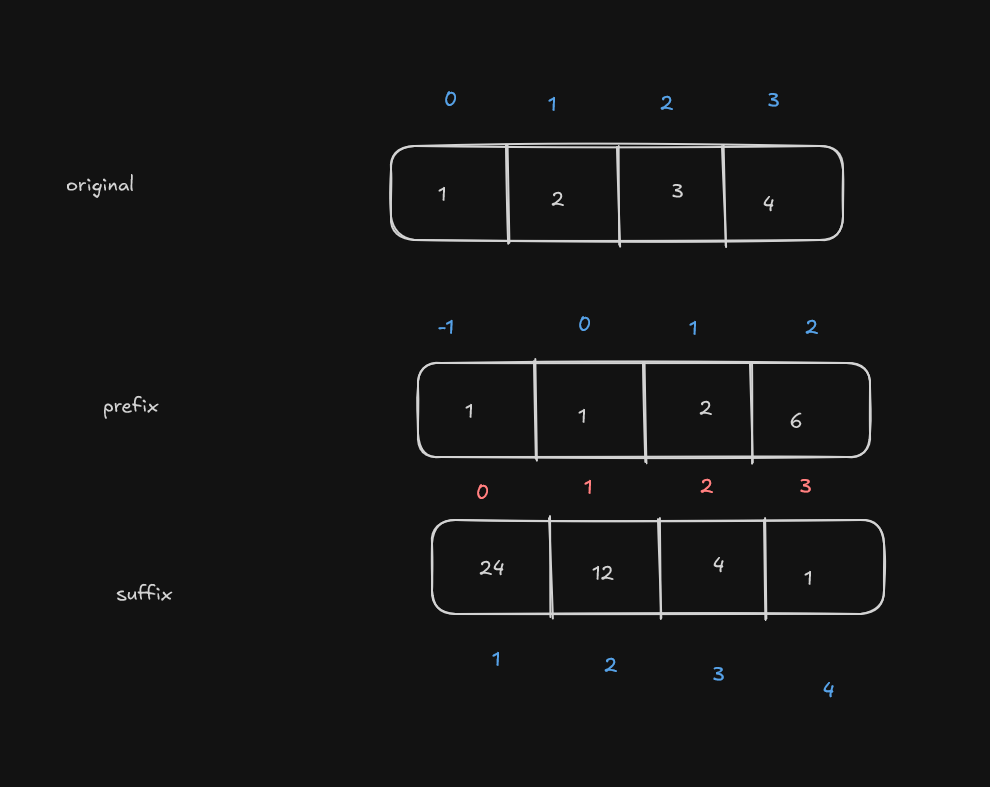
\includegraphics{1.png}
\end{figure}

\begin{figure}
		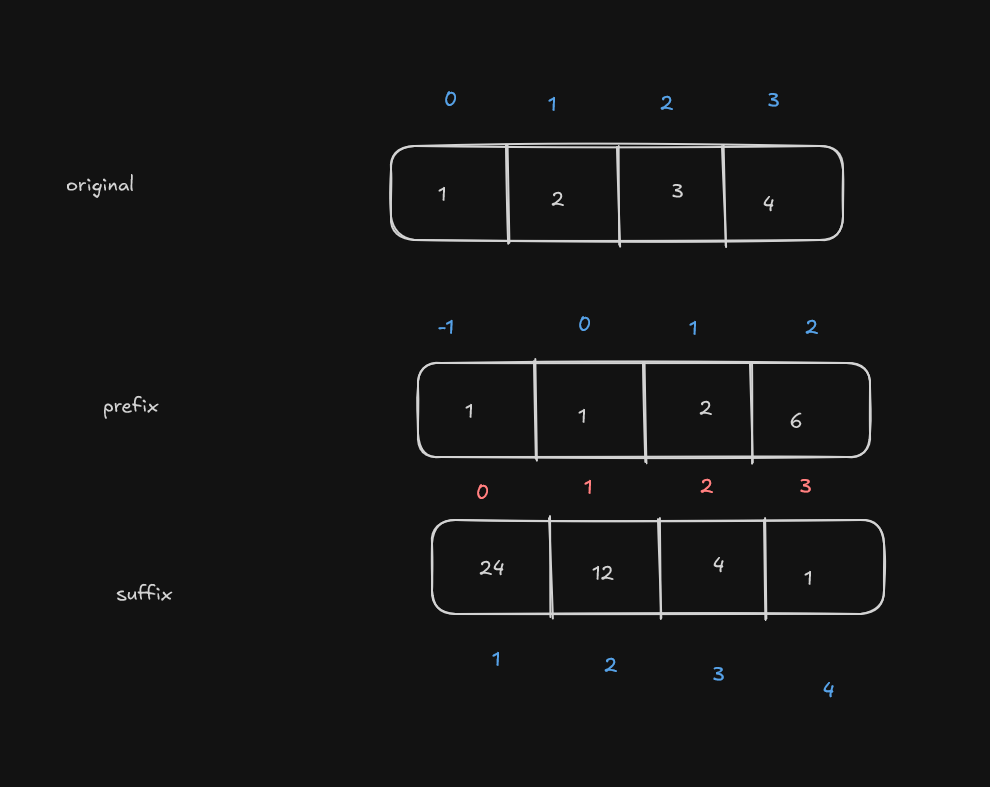
\includegraphics{1.eps}
\end{figure}

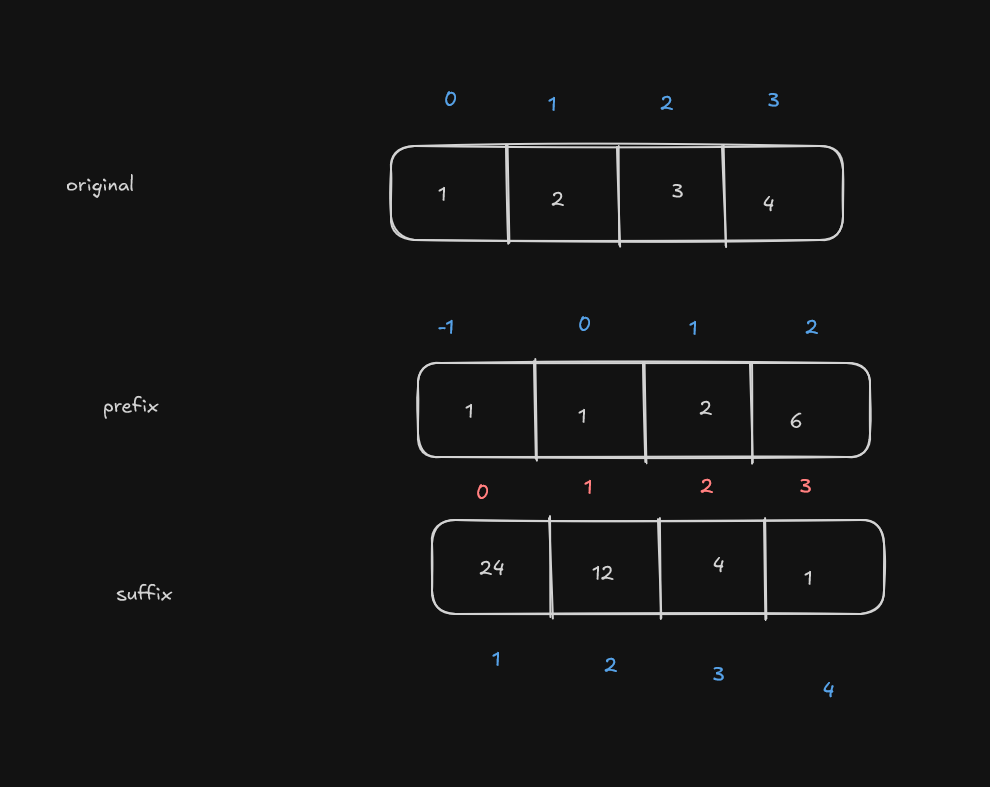
\includegraphics{1.eps}

\end{lstlisting}\\ \\


\chapter{Two Pointers}

\section{Explanation}

Having two pointers pointed at different parts of a string or an array. The pointers move from start and end closer to each other. Or they can move in the same direction

\section{When to use}
When we need to compare an element against other elements

\begin{itemize}
\item Comparing elements from two ends: Like checking for palindromes or finding pairs in a sorted array.
\item searching for a target sum or condition. In \textbf{"Two Sum"} where we need two numbers which meet a condition
\item Removing duplicates from sorted arrays
\item Finding subarrays like in \textbf{"Sliding Window"} problems
\end{itemize}	

\section{Example questions}
\begin{itemize}
\item Remove Duplicates From Sorted Array
\item Reverse String
\item Move Zeroes
\end{itemize}	
167, 15, 11


\include{Patterns/Fast and Slow Pointers}
141, 202, 287

\include{Patterns/Sliding Window} 
643, 3, 76

\include{Patterns/In-place Reversal of a LinkedList}
206, 92, 24

\include{Patterns/Monotonic Stack}
496, 739, 84


\include{Patterns/Top K Elements}
K Largest = Min - Heap
K Smallest = Max - Heap
215, 347, 373


\include{Patterns/Merge Intervals}
overlapping intervals
56, 57, 435

\section{Modified Binary Search}
\include{Patterns/Modified Binary Search}
33, 153, 240


\include{Patterns/Tree Breadth First Search}
102, 994, 127

\include{Patterns/Tree Depth First Search}
133, 113, 210

\include Binary Tree Traversal
257

InOrder
239

PostOrder
124

LevelOrder
107


\include{Patterns/Island}
733, 200, 130


\include{Patterns/Backtracking}
46, 78, 51

\include{Dynamic Programming}
COmmon Dp Patterns
1. Fibonaci Numbers
2. 0/1 Knapsack
3. Longest Common Subsequence
4. Longest Increasing Subsequence
5. Subset Sum
6. Matrix Chain Multiplication
70, 300, 322, 416, 1143, 312

\section{Cyclic Sort}
\include{Patterns/Cyclic Sort}

\section{Stack}
\chapter{Stack}

\section{Basics}
	\begin{itemize}
		\item Abstract data type that supports push and pop operations.
		\item Can be implemented using arrays and linked lists
		\item The behavior is often called LIFO( Last-In-First-Out)
		\item Used to implement \textbf{Depth-First-Search}
	\end{itemize}
	
	\section{Corner Cases}
		\begin{itemize}
			\item Empty stack. Popping from an empty stack
			\item Stack with one item
			\item Stack with two items
		\end{itemize}
		
	
	\section{Time complexity}
	
	\begin{center}
		\begin{tabular}{||c c||}
		\hline
		Operation & Complexity\\
		\hline\hline
		Top/Peek & O(1)\\
		\hline
		Push & O(1)\\
		\hline
		Pop & O(1)\\
		\hline
		isEmpty & O(1)\\
		\hline
		Search & O(n)\\
		\hline
			
		\end{tabular}
	\end{center}
	
	
	

\chapter{Hashmap}

\section{Questions}\\

Two Sum\\ \\
\href{https://leetcode.com/problems/two-sum/description/}{1. Two Sum}


\section{Example Usage}\\



\begin{lstlisting}
 public int[] TwoSum(int[] nums, int target)
 {
     var map = new Dictionary<int, int>();

     for (int i = 0; i < nums.Length; i++)
     {
         var diff = target - nums[i];
         if (map.ContainsKey(diff)) return [map[diff], i];
         map[nums[i]] = i;
     }
     throw new Exception();
 }
\end{lstlisting}\\ \\






\section{Graphs}
\include{Patterns/Graphs}



\section{Two Heaps}
\include{Patterns/Two Heaps}

\section{Subsets}
\include{Patterns/Subsets}



\section{Bitwise XOR}
\include{Patterns/Bitwise XOR}



\section{K-way Merge}
\include{Patterns/K-way Merge}


\chapter{Greedy Algorithm}

\section{Description}
A greedy algorithm makes an optimal choice at each step in the process, which then becomes the overall optimal choice.

\section{When to use}
A greedy algo can be implemented when some properties are in place
\begin{itemize}
\item Greedy Choice Property
	A global(overall) optimal solution can be reached by choosing the optimal choice at each step.
\end{itemize}

\section{Questions}

\href{https://leetcode.com/problems/best-time-to-buy-and-sell-stock/description/}{121. Best Time to Buy and Sell Stock}
 

 
\section{Example}

\begin{lstlisting}
 public int MaxProfit(int[] prices) {
var min = int.MaxValue;
var profit = 0;

    for(int i=0; i< prices.Length; i++){
        var currentProfit = prices[i] - min;
        profit = currentProfit > profit ? currentProfit: profit;

        min = min > prices[i] ? prices[i] : min;
    }
    return profit;
}
\end{lstlisting}




\section{0/1 Knapsack (Dynamic Programming)}
\include{Patterns/Knapsack}



\section{Trie}
\include{Patterns/Trie}

\section{Topological Sort (Graph)}
\include{Patterns/Topological Sort}

\section{Union Find}
\include{Patterns/Union Find}

\section{Ordered Set}
\include{Patterns/Ordered Set}

\section{Multi-thread}
\include{Patterns/Multi-thread}

